\chapter{Introduction}
\label{ch:Introduction}

\section{Background and Problem Statement}
\label{sec:BackgroundProblemStatement}
In recent years, the way people seek dermatological advice has changed significantly, mainly due to the COVID-19 pandemic. Teledermatology, a branch of telemedicine, has become a popular way to diagnose and manage skin conditions remotely. Telemedicine uses telecommunications technology to provide healthcare services from a distance, allowing patients to consult with healthcare providers without needing to be physically present. \par
\vspace{\baselineskip}
\begin{figure}[ht]
    \centering
    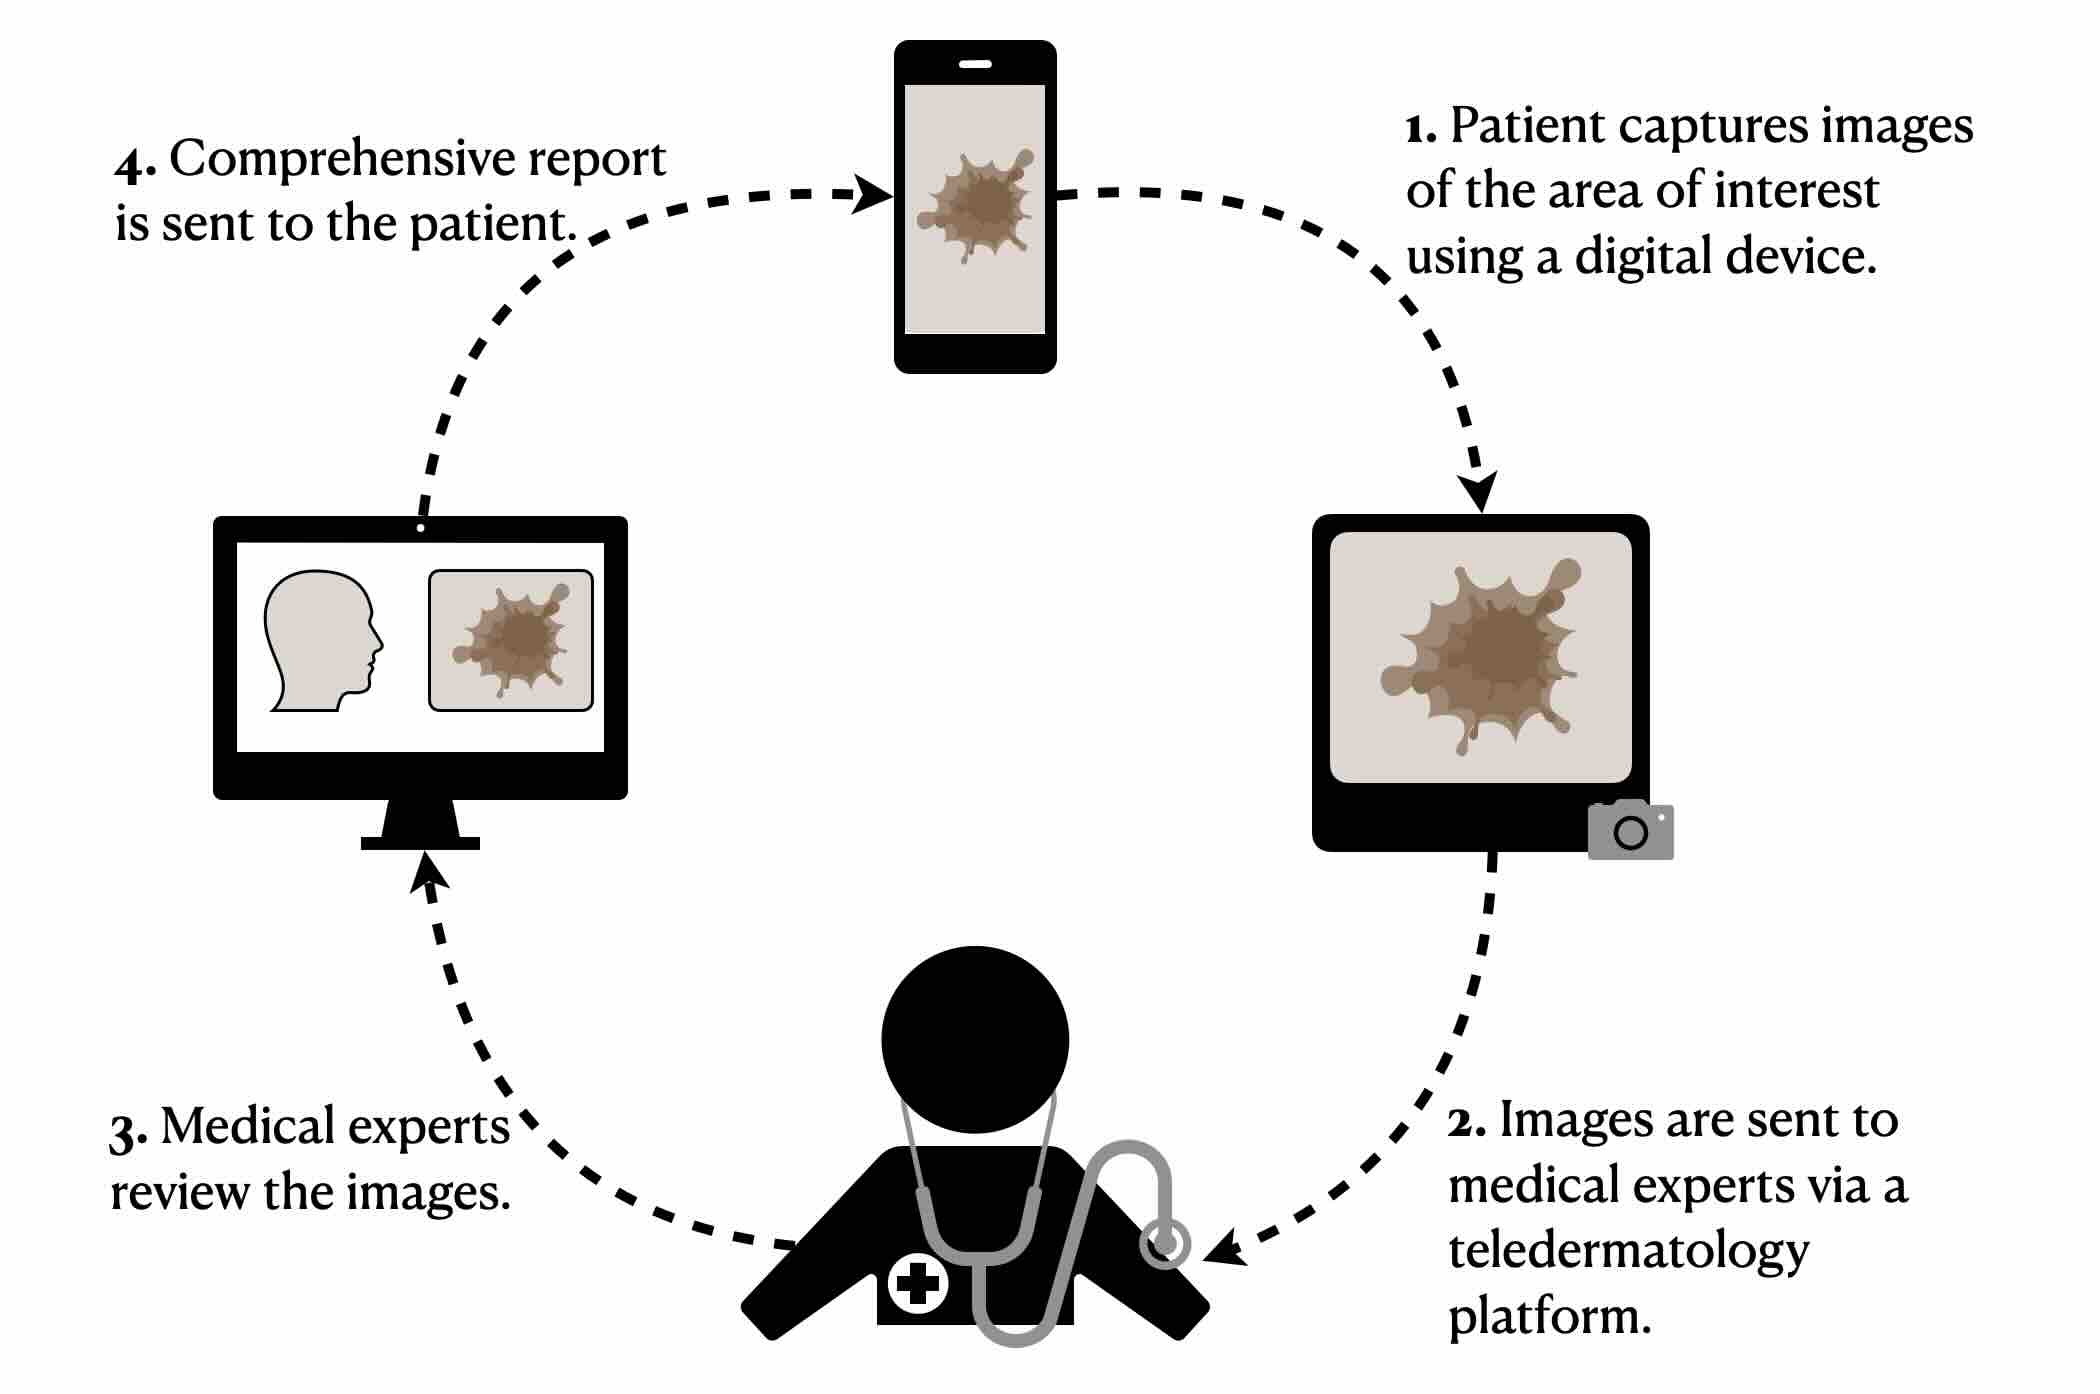
\includegraphics[keepaspectratio,width=14cm]{img/TD_workflow.jpg}
    \caption{This diagram shows the simplified process of a teledermatology consultation, starting from the patient capturing images of their skin condition to receiving a detailed medical report.}
    \label{fig:TD_workflow}
\end{figure}

\noindent
In teledermatology, patients use mobile applications to take pictures of their skin conditions with everyday devices like smartphones and tablets. These images are then sent to dermatologists for analysis, eliminating the need for face-to-face appointments. \autoref{fig:TD_workflow} shows each step in the teledermatology process, highlighting the essential role of image quality in ensuring accurate diagnosis and effective patient care. \par
\vspace{\baselineskip}
\noindent
However, the success of teledermatology relies heavily on the quality of the images patients capture. Despite the convenience of modern technology, many images sent by patients do not meet the necessary standards. Issues such as poor lighting, blurred images, and inadequate representation of skin conditions can greatly limit a dermatologist’s ability to make accurate diagnoses. These challenges with image quality reduce the effectiveness of teledermatology. \par
\vspace{\baselineskip}
\noindent
This common problem highlights the critical need to improve the quality of images taken through mobile applications. This thesis aims to address this problem by developing and implementing automated image quality assessment techniques to enhance the reliability and effectiveness of teledermatology. \par 


\section{Objectives of the Thesis}
\label{sec:Objectives}
The primary goal of this thesis is to develop and evaluate automated methods for assessing image quality within the context of teledermatology. The objectives are varied, starting with a comprehensive literature review of image quality assessment methods from the general imaging domain to determine their suitability for teledermatology applications. This thesis also aims to select appropriate quality metrics, apply these methods to relevant dermatological datasets, and create a reproducible repository for future research. \par
\vspace{\baselineskip}
The specific objectives of this thesis are detailed as follows:
\begin{itemize}
    \item An extensive review of the literature on image quality assessment (IQA) methods, focusing on their application in teledermatology.
    \item Identifying and selecting image quality metrics that are most suitable for assessing the quality of dermatological images.
    \item Evaluate the performance of selected image quality metrics on dermatological datasets to determine their effectiveness in assessing image quality.
    \item Develop a reproducible repository of image quality assessment tools and methodologies for teledermatology applications.
\end{itemize}
\noindent
Achieving these objectives will greatly improve the efficiency and accuracy of teledermatology services by creating a way to assess image quality. This improvement will streamline workflows, save time, and reduce frustration in teledermatology. By providing effective tools and methods for evaluating the quality of patient images remotely, this research will ultimately lead to better diagnostic accuracy and overall patient care in remote dermatological consultations. \par

\section{Organisation of this Thesis}
\label{sec:Structure}
This thesis is structured into six chapters to provide a clear and systematic exploration of image quality assessment in teledermatology. \autoref{ch:LiteratureReview} covers the literature review, discussing previous and related works on image quality assessment (IQA) and teledermatology. \autoref{ch:Methodology} details the methodologies, including those used in the literature review and those specific to IQA and teledermatology. In \autoref{ch:Implementation}, the experiments conducted are described, showing the approaches taken, along with the metrics used. \autoref{ch:ResultsAnalysis} presents the results of these investigations. Finally, \autoref{ch:DiscussionConclusion} concludes the thesis, summarizing the findings and suggesting directions for future research. \par
\vspace{\baselineskip}
\noindent
All figures and tables in this thesis are created by the author unless otherwise referenced. If any code is referenced, the path or module is provided in the footnotes. \par